\chapter{Implementation and Results}
In this section we cover the implementation of the project and the results.
The hardware used was the Virtex UltraScale+ FPGA VCU118 Board.
\begin{figure}[ht]
    \centering
    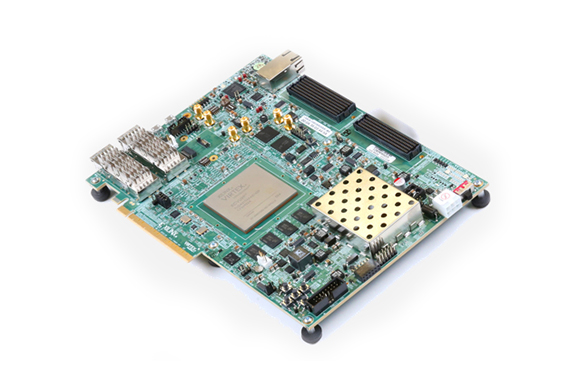
\includegraphics[width=0.8\linewidth]{img/board.jpg}
    \caption{VCU118 Board}%
    \label{fig:board}
\end{figure}

The project used the high-speed parallel to serial GTY transceiver built into
the VCU118 board. We looked to modify the functionality of a basic
implementation of the  transceiver.

The basic implementation is as follows:
There is a PRBS generator which feeds a series of bits to the transceiver. The
transceiver serializes them, then transmits the bits. 
On the reception side, the transceiver receives the bits, deserialises them,
then compares the recieved bits with a local PRBS generator.

